\documentclass[11pt,a4paper]{article}

\usepackage{filecontents}
\begin{filecontents*}{\jobname.bib}
  @misc{tracing,
    author = {{Tokio contributors}},
    title = {{tracing: application-level tracing for Rust}},
    year = {2024},
    howpublished = {\url{https://docs.rs/tracing}},
    note = {Accessed 12 June 2026}
  }
  @misc{tracingsub,
    author = {{Tokio contributors}},
    title = {{tracing-subscriber: utilities for implementing tracing subscribers}},
    year = {2024},
    howpublished = {\url{https://docs.rs/tracing-subscriber}},
    note = {Accessed 12 June 2026}
  }
  @misc{logfire,
    author = {{Pydantic}},
    title = {{Logfire: observability for Pydantic and beyond}},
    year = {2024},
    howpublished = {\url{https://logfire.pydantic.dev/docs/}},
    note = {Accessed 12 June 2026}
  }
  @misc{otel,
    author = {{OpenTelemetry Authors}},
    title = {{OpenTelemetry specification}},
    year = {2024},
    howpublished = {\url{https://opentelemetry.io/docs/specs/otel/}},
    note = {Accessed 12 June 2026}
  }
  @misc{tracingotel,
    author = {{Tokio contributors}},
    title = {{tracing-opentelemetry: integration between tracing and OpenTelemetry}},
    year = {2024},
    howpublished = {\url{https://docs.rs/tracing-opentelemetry}},
    note = {Accessed 12 June 2026}
  }
  @misc{otlpsdk,
    author = {{OpenTelemetry Authors}},
    title = {{opentelemetry-otlp: OTLP exporters for the Rust SDK}},
    year = {2024},
    howpublished = {\url{https://docs.rs/opentelemetry-otlp}},
    note = {Accessed 22 June 2026}
  }
  @misc{loki,
    author = {{Grafana Labs}},
    title = {{Grafana Loki: like Prometheus, but for logs}},
    year = {2024},
    howpublished = {\url{https://grafana.com/oss/loki/}},
    note = {Accessed 22 June 2026}
  }
  @misc{otelcol,
    author = {{OpenTelemetry Authors}},
    title = {{OpenTelemetry Collector}},
    year = {2024},
    howpublished = {\url{https://opentelemetry.io/docs/collector/}},
    note = {Accessed 22 June 2026}
  }
\end{filecontents*}

\usepackage[margin=2.5cm]{geometry}
\usepackage{fontspec}
\setmainfont{Latin Modern Roman}
\setsansfont{Latin Modern Sans}
\setmonofont{Hack}[Scale=0.85]
\usepackage{amssymb}
\usepackage{amsmath}
\usepackage{graphicx}
\usepackage[dvipsnames,table]{xcolor}
\usepackage{tikz}
\usetikzlibrary{positioning,arrows.meta,fit,backgrounds,shapes.geometric,calc,decorations.pathmorphing}
\usepackage{listings}
\usepackage{enumitem}
\usepackage{hyperref}
\usepackage{fancyhdr}
\usepackage{titlesec}
\usepackage{parskip}
\usepackage{float}
\usepackage{booktabs}
\usepackage{array}
\usepackage{adjustbox}
\usepackage[numbers,square,sort&compress]{natbib}
\usepackage{microtype}
\usepackage[most]{tcolorbox}

% Colors (mirroring the sibling DVerse documents)
\definecolor{router}{HTML}{E74C3C}
\definecolor{peer}{HTML}{3498DB}
\definecolor{client}{HTML}{2ECC71}
\definecolor{agent}{HTML}{3498DB}
\definecolor{machine}{HTML}{ECF0F1}
\definecolor{cipher}{HTML}{9B59B6}
\definecolor{session}{HTML}{3498DB}
\definecolor{codebg}{HTML}{F8F8F8}
\definecolor{codeframe}{HTML}{DDDDDD}
\definecolor{nixblue}{HTML}{5277C3}
\definecolor{soft}{HTML}{F4F6F8}

% Abstract box
\newtcolorbox{abstractbox}[1][]{
  enhanced, colback=soft, colframe=nixblue,
  boxrule=0.6pt, arc=2pt, left=10pt, right=10pt, top=8pt, bottom=8pt,
  title=\textbf{Abstract}, coltitle=white, colbacktitle=nixblue,
  fonttitle=\sffamily\bfseries, #1
}

% Listings style
\lstset{
  basicstyle=\ttfamily\small,
  backgroundcolor=\color{codebg},
  frame=single,
  rulecolor=\color{codeframe},
  breaklines=true,
  breakatwhitespace=true,
  tabsize=2,
  showstringspaces=false,
  keywordstyle=\color{blue},
  stringstyle=\color{red!70!black},
  commentstyle=\color{green!50!black},
}

\pagestyle{fancy}
\fancyhf{}
\fancyhead[L]{\small\textit{Structured logging across the DVerse workspace}}
\fancyhead[R]{\small\textit{DVerse Platform}}
\fancyfoot[C]{\thepage}
\renewcommand{\headrulewidth}{0.4pt}

\hypersetup{
  colorlinks=true,
  linkcolor=blue!60!black,
  urlcolor=blue!60!black,
  citecolor=blue!60!black,
}

\title{%
  \vspace{-1cm}
  {\LARGE\bfseries Structured Logging Across the DVerse Workspace:\\
  Connecting the Rust Platform to the Chat-App Observability Pipeline}
}
\author{Yordan Mitev}
\date{\today}

\begin{document}
\sloppy
\maketitle
\thispagestyle{fancy}

\begin{abstractbox}
  The DVerse Rust workspace and the chat-app Python backend
  evolved separately and accumulated incompatible logging habits:
  the chat-app already had a fully wired observability pipeline
  (Logfire, OpenTelemetry, Jaeger, Prometheus, Grafana) authored
  by Abel, while the Rust side scattered diagnostics across
  \texttt{eprintln!}, \texttt{println!}, and an in-app
  \texttt{push\_log} sink. This document describes the work that
  moved every diagnostic in the Rust workspace through a single
  \texttt{tracing} subscriber, gave each event named fields, and
  then wired those events into the same observability pipeline
  via OTLP. A new \texttt{dverse-obs} crate now installs the
  subscriber for every binary, exports logs and traces over OTLP
  to the chat-app's collector, and bakes a profile-based default
  endpoint (\texttt{localhost} in debug builds, the central
  dverse sink in release builds) so the binaries are
  zero-configuration in the developer loop.
\end{abstractbox}

\vspace{1em}

\begin{table}[H]
  \centering
  \small
  \begin{tabular}{|l|l|p{7.5cm}|}
    \hline
    \rowcolor{gray!15}
    \textbf{Version} & \textbf{Date} & \textbf{Changes} \\
    \hline
    V1 & 21 June 2026 & Initial writeup of the structured-logging
    rollout across the Rust workspace: the shared
    \texttt{dverse-obs} crate, the OTLP integration that moved
    the slogs into Loki and Jaeger via the chat-app collector,
    the profile-based default endpoint, and the router's GUI
    sink preserved alongside OTLP export. \\
    \hline
  \end{tabular}
  \caption{Revision history.}
  \label{tab:logging-history}
\end{table}

\newpage
\tableofcontents

\newpage
% ==============================================================
\section{Introduction}
% ==============================================================

The DVerse platform is split across two halves of the
repository. The Rust workspace under \texttt{src/} hosts the
Zenoh router, the Tauri desktop launcher, the
\texttt{bot\_framework} crate, and the demo agents. The Python
project under \texttt{experiments/chat-app/} hosts the FastAPI
backend, the standalone bot agents, and the docker-compose
telemetry stack. Both halves communicate over the same Zenoh
fabric, but they were built by different people at different
times and ended up with very different logging habits.

The chat-app side already had a finished observability pipeline.
Abel had wired Logfire for structured logging and instrumented
the backend with OpenTelemetry, exporting traces to Jaeger and
metrics to Prometheus, with Grafana dashboards on top. Every HTTP
request, every LLM call, every A2A turn was already a structured
event with named fields and a service identifier. Restarting the
stack was a single \texttt{docker compose up}.

The Rust side had nothing comparable. Diagnostics were a mix of
\texttt{println!}, \texttt{eprintln!}, and an in-app
\texttt{AppState::push\_log} buffer that the router GUI rendered
to a log panel. Every call site that wanted to be visible in both
stderr and the GUI had to write the message twice. The mTLS
handshake errors that Zenoh and rustls emit through their own
\texttt{tracing} events were silently dropped, because no
subscriber was installed to consume them. The result was that
real failures (an unauthorised client, a missing client cert on
an outbound link) were invisible until somebody read the source
by hand.

This document covers the work that brought the Rust workspace up
to the same observability standard, and explains how that change
positions the platform for one shared pipeline across both halves
of the codebase.

\subsection{Scope}

The structured-logging rollout has four parts:

\begin{itemize}
  \item A shared subscriber installation in the new
        \texttt{dverse-obs} crate, used by every binary that
        does not need a GUI sink.
  \item A router-specific entry point in the same crate
        (\texttt{init\_with\_extra\_layer}) that lets the router
        keep its custom \texttt{tracing\_subscriber::Layer}
        feeding the desktop log panel while still going through
        the shared subscriber.
  \item A workspace-wide migration of \texttt{println!},
        \texttt{eprintln!}, and \texttt{push\_log} calls to
        \texttt{tracing::info!} / \texttt{warn!} / \texttt{error!}
        with named structured fields.
  \item An OTLP exporter inside \texttt{dverse-obs} that ships
        every event to the chat-app's collector, with a
        profile-baked default endpoint so the developer loop
        works with zero configuration.
\end{itemize}

This document treats those pieces together because they were
delivered in one PR and only make sense in combination. It also
explains why the resulting log surface is shape-compatible with
the chat-app's existing pipeline and how the OTLP wiring made
that compatibility concrete instead of theoretical.

% ==============================================================
\section{The Chat-App Pipeline We Encountered}
% ==============================================================

The chat-app pipeline was not designed against requirements we
wrote. It was already there when the team started thinking about
observability for the Rust side, and inheriting its conventions
was cheaper than designing a parallel system. The shape of the
pipeline is:

\begin{itemize}
  \item \textbf{Structured logging} via Logfire, configured once
        at startup in \texttt{backend/observability.py}. Records
        every Pydantic model, every LLM call, every Anthropic
        request. Scrubbing patterns redact
        \texttt{password\_hash} and \texttt{access\_token} fields
        before serialisation.
  \item \textbf{Distributed tracing} via OpenTelemetry, with the
        OTLP HTTP exporter pointed at a collector inside the same
        compose project. The collector forwards traces to Jaeger
        and metrics to Prometheus. The instrumented call sites
        live in \texttt{backend/telemetry.py} and produce
        histograms for HTTP latency, LLM duration, Zenoh
        round-trip, and A2A turn duration.
  \item \textbf{Visualisation} via a Grafana dashboard with four
        sections (HTTP API, LLM Calls, Zenoh Bot, A2A Council),
        provisioned automatically from
        \texttt{grafana/provisioning/}.
  \item \textbf{A working development loop} where the entire
        stack (router, Ollama, Jaeger, OTel collector,
        Prometheus, Grafana) is brought up by
        \texttt{docker compose up}.
\end{itemize}

Encountering this pipeline raised the bar for the Rust side. Any
log line the Rust workspace produced needed to at least be a
candidate for the same kind of analysis: filtered by named
fields, sliced by service, comparable across runs. The free-text
\texttt{eprintln!} calls on the Rust side were not.

% ==============================================================
\section{What Structured Logging Means Here}
% ==============================================================

Structured logging in this context means three things at once,
each of which the chat-app pipeline already assumed:

\begin{enumerate}
  \item Every diagnostic is an \emph{event} with a level, a
        target (the module that emitted it), a literal message,
        and zero or more named fields with typed values.
  \item Events flow through a single in-process subscriber that
        applies filters and routes them to one or more
        \emph{layers}: a stderr formatter, a GUI buffer, a remote
        exporter, etc.
  \item Verbosity is controlled by environment variables, not by
        editing call sites. Cranking up the
        \texttt{zenoh::transport} target to \texttt{trace} for
        ten minutes does not require a recompile.
\end{enumerate}

The Rust ecosystem's \texttt{tracing} crate matches that shape
exactly. The Python side already used Logfire, which itself
emits OpenTelemetry spans and structured log records. Converging
on \texttt{tracing} on the Rust side was the cheapest way to
make the two halves emit comparable events.

% ==============================================================
\section{The Rust-Side Implementation}
% ==============================================================

The implementation is small. Two modules and a workspace-wide
sweep of call sites.

\subsection{\texttt{bot\_framework::logging}}

This module owns the default subscriber installation used by
every binary that does not need a custom layer (the demo agents,
the framework CLI, the launcher's headless modes). It exposes
\texttt{init()}, which is idempotent and safe to call from any
\texttt{main()} without coordination. The function reads
\texttt{RUST\_LOG} if set, otherwise applies a built-in default
filter that keeps our own crates at \texttt{info} and pins noisy
transitive crates (\texttt{zenoh}, \texttt{rustls},
\texttt{mio}, \texttt{hyper}, \texttt{reqwest}, \texttt{zbus})
at \texttt{warn}. The fmt layer writes to stderr so stdout stays
clean for any pipeline-like use of the binary.

The default filter lives in this module as a single public
constant. The router used to duplicate the filter in its own
module with a comment saying the two were ``kept in sync
intentionally''. Nothing enforced the invariant and the two
would silently drift the moment one was edited. The cleanup
followed review feedback on the original PR.

\subsection{\texttt{zenoh\_router::logging}}

The router cannot use the shared \texttt{init()} unchanged
because it has a GUI sink. The desktop window has a log panel
that renders entries from \texttt{AppState.log}; before the
rollout, every interesting call site wrote to
\texttt{AppState.log} directly and to stderr separately. The
router-side module installs its own subscriber with two layers
stacked on the same global registry:

\begin{itemize}
  \item The standard fmt layer (stderr, full level / target /
        fields), identical to the one
        \texttt{bot\_framework::logging::init} installs.
  \item A custom \texttt{GuiLogLayer} that implements
        \texttt{tracing\_subscriber::Layer}, renders each event to
        a single line, prefixes \texttt{[WARN]} or \texttt{[ERROR]}
        so the GUI panel is scannable without colour, and pushes
        the rendered line into \texttt{AppState.log} via
        \texttt{try\_lock}.
\end{itemize}

The \texttt{try\_lock} matters. The layer is invoked from every
thread that emits a tracing event, and a few of those code paths
already hold the \texttt{AppState} mutex when they emit. A
blocking \texttt{lock} would deadlock; \texttt{try\_lock}
degrades to ``write this one to stderr only'' instead, which the
fmt layer is already doing. Correctness is preserved under
contention at the price of occasionally missing a line from the
GUI panel, which is the right trade-off for a log surface.

Both layers receive every event that passes the env filter, so
one call site produces both a stderr line and a GUI line without
duplication.

\subsection{The Sweep of Call Sites}

Every previous \texttt{push\_log} / \texttt{eprintln!} /
\texttt{println!} that was diagnostic was rewritten to a
\texttt{tracing} macro with structured fields. Numbers and IPs
that used to be embedded in the format string became named
fields. A line that previously read

\begin{lstlisting}
eprintln!("admitted {} from {}", cn, endpoint);
\end{lstlisting}

\noindent became

\begin{lstlisting}
tracing::info!(cn = %cn, endpoint = %endpoint, "admitted operator");
\end{lstlisting}

\noindent The literal message is now stable across runs, and
\texttt{cn} and \texttt{endpoint} are filterable by any layer
downstream. A few \texttt{println!} calls in the framework CLI
were kept, because they are user-facing stdout output (the path
of an issued certificate, the ZID of an opened session) and not
log lines.

\texttt{AppState::push\_log} dropped its own \texttt{eprintln!}
inside the rollout, because the fmt layer already writes to
stderr. The method is now an internal sink invoked only by
\texttt{GuiLogLayer}.

% ==============================================================
\section{How This Connects to the Chat-App Pipeline}
% ==============================================================

The Rust workspace now exports to the chat-app's OTLP collector
through the same \texttt{dverse-obs} subscriber every binary
uses. The wire format Logfire and the Python OTel SDK already
emit is the same OTLP that \texttt{opentelemetry-otlp} produces
from Rust, so the two halves of the platform meet on a single
collector without either side translating the other's
events. The implementation lives one section further down; this
section is about why it was the right thing to converge on.

The structured fields on the Rust side are the part that turns
that integration from a bridge into something useful. A Grafana
panel filtering ``Zenoh Bot round-trip latency by bot name'' is
only possible because the Python side records the bot name as a
field. The Rust side now does the same thing for its own events
(\texttt{cn=}, \texttt{endpoint=}, \texttt{session=}). The two
sides converge on the same shape without one side rewriting the
other's emissions.

The other shape-compatibility property is the verbosity contract.
Both sides expect verbosity to be controlled by environment
variables (\texttt{LOGFIRE\_*} and \texttt{OTEL\_*} on the
Python side, \texttt{RUST\_LOG} on the Rust side), and both
default to quiet. Operators do not have to learn two ways of
turning logging up.

% ==============================================================
\section{Wiring the OTLP Exporter}
% ==============================================================

Remote shipping lives in the new \texttt{dverse-obs} crate, in
the Loki sink added to the chat-app's OTel collector, and in
the Grafana datasource provisioned alongside it. A fresh
\texttt{cargo run -p dverse-ping} on a developer's machine
appears in Grafana within ten seconds, queryable as
\texttt{\{service\_name="dverse-ping"\}}, alongside the
chat-app's own backend spans and metrics.

\subsection{The \texttt{dverse-obs} Crate}

\texttt{dverse-obs} is a leaf crate under \texttt{src/dverse\_obs/}.
It exposes two entry points, both idempotent:

\begin{itemize}
  \item \texttt{init(service\_name)} for the common case. Every
        dverse binary calls it from \texttt{main()} with its own
        identifier (\texttt{"dverse-ping"}, \texttt{"dverse-pong"},
        and so on).
  \item \texttt{init\_with\_extra\_layer(service\_name, extra)}
        for binaries that need an additional
        \texttt{tracing-subscriber} layer. The router is the
        only current caller; it passes its
        \texttt{GuiLogLayer} so the desktop log panel keeps
        getting fed from the same global subscriber that exports
        to OTLP.
\end{itemize}

Internally the crate installs:

\begin{enumerate}
  \item An \texttt{EnvFilter} honouring \texttt{RUST\_LOG} with
        the workspace's existing default filter
        (\texttt{DEFAULT\_FILTER}).
  \item A compact \texttt{fmt} layer writing to stderr so the
        local \texttt{cargo run} workflow is unchanged.
  \item An \texttt{opentelemetry-appender-tracing} bridge that
        forwards every \texttt{tracing} event to an OTLP logs
        exporter.
  \item A \texttt{tracing-opentelemetry} layer that exports
        spans over OTLP traces.
\end{enumerate}

Items (3) and (4) are powered by
\texttt{opentelemetry-otlp} over its Tonic (gRPC)
transport. The resource attribute \texttt{service.name} defaults
to the value passed into \texttt{init}, override-able via
\texttt{OTEL\_SERVICE\_NAME}, matching the convention the
chat-app's \texttt{backend/telemetry.py} already uses.

\subsection{Profile-Based Default Endpoint}

The crate ships a compile-time fallback for
\texttt{OTEL\_EXPORTER\_OTLP\_ENDPOINT}, keyed off the build
profile via \texttt{cfg(debug\_assertions)}:

\begin{itemize}
  \item Debug builds (\texttt{cargo run},
        \texttt{cargo build}, every workspace test) default to
        \texttt{http://localhost:4317}, the chat-app collector
        when its docker-compose stack is up.
  \item Release builds (\texttt{cargo build -{}-release})
        default to
        \texttt{https://logs.\allowbreak dverse.\allowbreak yordanmitev.\allowbreak me:4317},
        the central dverse sink. The sink is not hosted yet but
        the address is reserved so any binary shipped from this
        workspace lands in the production stream by default once
        the collector exists.
\end{itemize}

The environment variable still wins when set, and the empty
string is an explicit opt-out (skip the OTLP branch entirely),
which is the escape hatch for CI runs and air-gapped boxes
where periodic connection-refused warnings would be noise. The
endpoint is passed to the SDK exporters via
\texttt{WithExportConfig::with\_endpoint} rather than by
mutating the process environment, so the profile default works
without surprises in multi-threaded \texttt{main()}s.

Figure~\ref{fig:obs-data-flow} shows the path a single
\texttt{tracing::info!} on the Rust side takes to a Grafana
panel.

\begin{figure}[H]
  \centering
  \begin{adjustbox}{max width=\textwidth}
  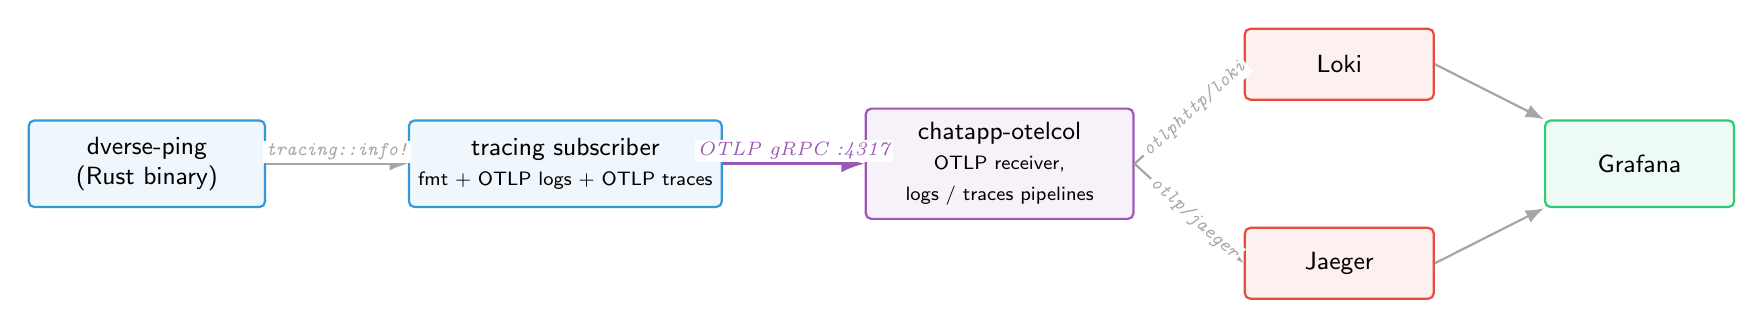
\begin{tikzpicture}[
      font=\small\sffamily,
      box/.style={draw, rounded corners=2pt, thick,
                  minimum width=3.0cm, minimum height=11mm,
                  align=center, fill=white},
      service/.style={box, draw=peer, fill=peer!8},
      stack/.style={box, draw=session, fill=session!8,
                    minimum width=3.8cm},
      collector/.style={box, draw=cipher, fill=cipher!8,
                        minimum width=3.4cm, minimum height=14mm},
      sink/.style={box, draw=router, fill=router!8,
                   minimum width=2.4cm, minimum height=9mm},
      ui/.style={box, draw=client, fill=client!8,
                 minimum width=2.4cm},
      flow/.style={-Latex, thick, gray!70},
      hot/.style={-Latex, very thick, cipher},
      lbl/.style={font=\scriptsize\itshape, fill=white, inner sep=1pt}
    ]

    \node[service] (rust) {dverse-ping\\(Rust binary)};
    \node[stack, right=18mm of rust] (stack)
      {tracing subscriber\\\scriptsize fmt + OTLP logs + OTLP traces};
    \node[collector, right=18mm of stack] (col)
      {chatapp-otelcol\\\scriptsize OTLP receiver,\\\scriptsize logs / traces pipelines};

    % Sink fan-out: Loki above and Jaeger below a coordinate
    % well to the right of the collector, so the labels on the
    % two diverging arrows have room to breathe.
    \coordinate (sinkmid) at ([xshift=26mm]col.east);
    \node[sink, above=8mm of sinkmid] (loki)   {Loki};
    \node[sink, below=8mm of sinkmid] (jaeger) {Jaeger};

    \node[ui, right=26mm of sinkmid] (grafana) {Grafana};

    \draw[flow] (rust) -- node[lbl, above] {\texttt{tracing::info!}} (stack);
    \draw[hot]  (stack) -- node[lbl, above] {OTLP gRPC :4317} (col);
    \draw[flow] (col.east) -- node[lbl, sloped, pos=0.55] {\texttt{otlphttp/loki}} (loki.west);
    \draw[flow] (col.east) -- node[lbl, sloped, pos=0.55] {\texttt{otlp/jaeger}} (jaeger.west);
    \draw[flow] (loki.east)   -- (grafana.north west);
    \draw[flow] (jaeger.east) -- (grafana.south west);

  \end{tikzpicture}
  \end{adjustbox}
  \caption{An event from a Rust binary on the developer's host
    reaches Grafana by going through the in-process subscriber,
    OTLP gRPC on port 4317 to the chat-app collector running in
    docker-compose, and the collector's logs and traces
    pipelines into Loki and Jaeger respectively. Grafana queries
    both as provisioned datasources.}
  \label{fig:obs-data-flow}
\end{figure}

\subsection{Per-Service \texttt{service.name} and the Router's GUI Sink}

Every workspace binary calls \texttt{dverse-obs} with its own
identifier (\texttt{dverse-ping}, \texttt{dverse-pong},
\texttt{dverse-router}, \texttt{dverse-bot-framework},
\texttt{dverse-launcher}, and the A2A council services), so each
one appears as a distinct \texttt{service.name} in Loki and
Jaeger. The earlier \texttt{bot\_framework::logging::init()}
remains as a thin shim that delegates to \texttt{dverse-obs} for
the benefit of out-of-tree callers, but the workspace binaries
no longer rely on its default.

The router is the interesting case because it cannot just call
\texttt{init}. Its desktop log panel needs its own
\texttt{GuiLogLayer}, and \texttt{tracing} allows exactly one
global subscriber per process. The original rollout solved this
with a router-specific \texttt{init\_with\_gui\_sink} that
duplicated the fmt-plus-filter stack. To bring the router into
the OTLP pipeline without re-introducing duplication,
\texttt{dverse-obs} exposes
\texttt{init\_with\_extra\_layer<L>(service\_name, extra)}. The
extra layer is boxed
(\texttt{Box<dyn Layer<Registry> + Send + Sync>}) and added at
the bottom of the registry stack, so it sees every event before
the filter drops or the formatter renders. The router's
\texttt{init\_with\_gui\_sink} is now a one-liner:

\begin{lstlisting}
dverse_obs::init_with_extra_layer(
    "dverse-router",
    GuiLogLayer { state },
);
\end{lstlisting}

\subsection{Chat-App Side: Loki and the otelcol Logs Pipeline}

The chat-app's collector was already configured for traces (to
Jaeger) and metrics (to Prometheus). It was missing a logs sink.
The PR adds Grafana Loki to
\texttt{experiments/chat-app/docker-compose.yml}, an
\texttt{otlphttp/loki} exporter and a \texttt{logs} pipeline to
\texttt{otel-collector-config.yaml}, and a Loki
datasource under
\texttt{experiments/chat-app/grafana/provisioning/datasources/}.
Loki's 3.x default config accepts OTLP receive on
\texttt{/otlp} out of the box and auto-maps OTel
\texttt{service.name} to its own \texttt{service\_name} label,
which is why the LogQL query in the abstract works without
extra relabelling.

The PR also removes a pre-existing duplicate \texttt{frontend:}
service definition that older docker compose versions tolerated
silently but v5 refuses to parse. That was a drive-by needed to
get the obs stack to come up at all on the reviewer's machine.

Figure~\ref{fig:endpoint-resolution} shows the decision flow
that the crate runs every time \texttt{init} is called.

\begin{figure}[H]
  \centering
  \begin{adjustbox}{max width=\textwidth}
  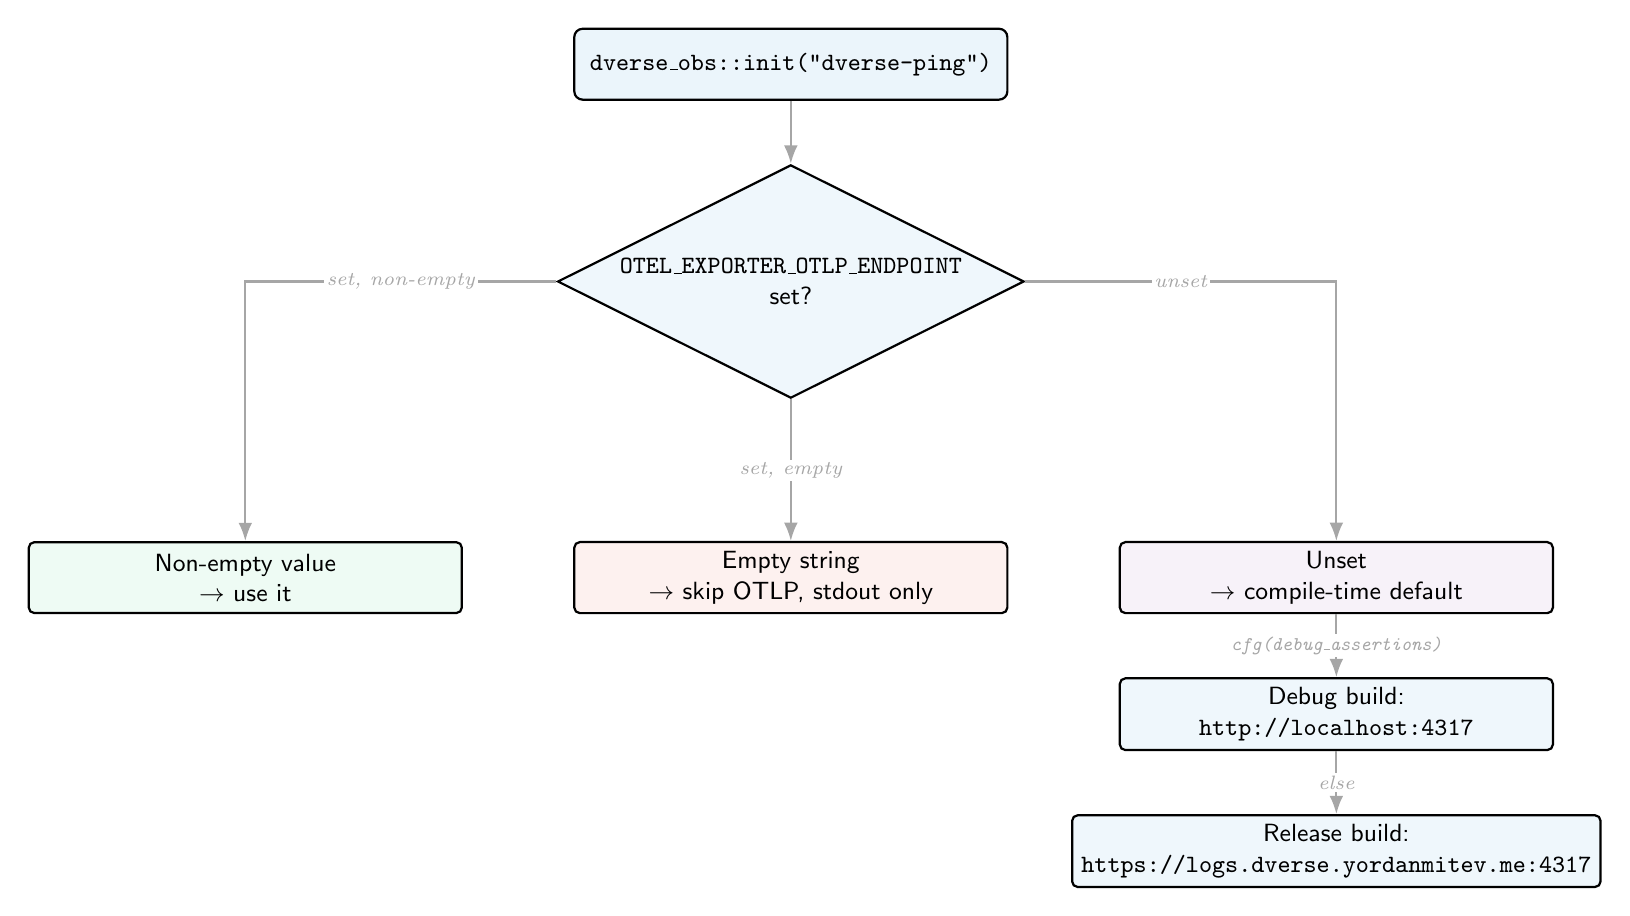
\begin{tikzpicture}[
      font=\small\sffamily,
      node distance=8mm,
      start/.style={draw, rounded corners=3pt, thick, fill=session!10,
                    minimum width=5.5cm, minimum height=9mm, align=center},
      decision/.style={draw, diamond, aspect=2, thick, fill=peer!8,
                       inner sep=2pt, align=center, minimum width=4.5cm},
      action/.style={draw, rounded corners=2pt, thick, fill=client!8,
                     minimum width=5.5cm, minimum height=9mm, align=center},
      opt/.style={draw, rounded corners=2pt, thick, fill=router!8,
                  minimum width=5.5cm, minimum height=9mm, align=center},
      def/.style={draw, rounded corners=2pt, thick, fill=cipher!8,
                  minimum width=5.5cm, minimum height=9mm, align=center},
      flow/.style={-Latex, thick, gray!70},
      lbl/.style={font=\scriptsize\itshape, fill=white, inner sep=1pt}
    ]

    \node[start] (init) {\texttt{dverse\_obs::init("dverse-ping")}};
    \node[decision, below=of init] (env)
      {\texttt{OTEL\_EXPORTER\_OTLP\_ENDPOINT}\\set?};
    \node[opt, below=18mm of env] (empty)
      {Empty string\\$\rightarrow$ skip OTLP, stdout only};
    \node[action, left=14mm of empty] (user)
      {Non-empty value\\$\rightarrow$ use it};
    \node[def, right=14mm of empty] (default)
      {Unset\\$\rightarrow$ compile-time default};
    \node[draw, rounded corners=2pt, thick, fill=session!8,
          minimum width=5.5cm, minimum height=9mm, align=center,
          below=of default] (debug)
      {Debug build:\\\texttt{http://localhost:4317}};
    \node[draw, rounded corners=2pt, thick, fill=session!8,
          minimum width=5.5cm, minimum height=9mm, align=center,
          below=of debug] (release)
      {Release build:\\\texttt{https://logs.dverse.yordanmitev.me:4317}};

    \draw[flow] (init) -- (env);
    \draw[flow] (env.west)  -| node[lbl, near start] {set, non-empty} (user.north);
    \draw[flow] (env.south) -- node[lbl] {set, empty} (empty.north);
    \draw[flow] (env.east)  -| node[lbl, near start] {unset} (default.north);
    \draw[flow] (default.south) -- node[lbl] {\texttt{cfg(debug\_assertions)}} (debug.north);
    \draw[flow] (debug.south) -- node[lbl] {else} (release.north);

  \end{tikzpicture}
  \end{adjustbox}
  \caption{Endpoint resolution inside
    \texttt{dverse\_obs::init}. The environment variable wins
    when set, the empty string is an explicit opt-out, and the
    unset case falls through to the profile-baked
    \texttt{DEFAULT\_OTLP\_ENDPOINT}.}
  \label{fig:endpoint-resolution}
\end{figure}

\end{document}
